% document formatting
\documentclass[10pt]{article}
\usepackage[utf8]{inputenc}
\usepackage[left=1in,right=1in,top=1in,bottom=1in]{geometry}
\usepackage[T1]{fontenc}
\usepackage{xcolor}

% math symbols, etc.
\usepackage{amsmath, amsfonts, amssymb, amsthm}

% lists
\usepackage{enumerate}

% images
\usepackage{graphicx} % for images

% code blocks
\usepackage{minted, listings} 

% verbatim greek
\usepackage{alphabeta}

\graphicspath{{./assets/images}}

\newcommand{\solution}{\textbf{Solution:}} 
\newcommand{\example}{\textbf{Example: }}

\title{EC ENGR 102 Week 1}

\author{Aidan Jan}
\date{\today}

\begin{document}
\maketitle
\subsection*{The Unit Step Function}
The unit step function denoted by $u(t)$ in this class, is given by:
\[u(t) = \begin{cases} 1 & t \geq 0 \\ 0 & t < 0 \end{cases}\]
It is also called the Heavyside step function.  Drawn below:
\begin{center}
    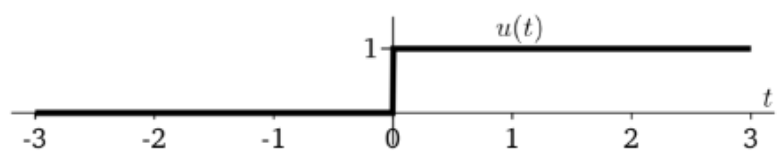
\includegraphics[scale=0.9]{W2_1.png}
\end{center}
\example\\
Suppose I wanted to write
\[x(t) = \begin{cases}e^{-t} & t \geq 1 \\ 0 & t < 1\end{cases}\]
We can do that in terms of the unit step function as
\[x(t) = e^{-t} u(t - 1)\]
\subsubsection*{The Unit Rectangle}
There are two definitions:
\begin{enumerate}
    \item \[rect(t) = \begin{cases} 1 & \vert t \vert < \frac{1}{2} \\ 0 & \text{else} \end{cases}\]
    \begin{itemize}
        \item This is a rectangle with height 1, from t = -0.5 to t = 0.5.
        \item Notice the area under the curve is 1.
    \end{itemize}
    \item \[rect_{\Delta}(t) = \begin{cases} \frac{1}{\Delta} & \vert t \vert < \frac{\Delta}{2}  \\ 0 & \text{else}\end{cases}\]
    \begin{itemize}
        \item This is a general case of the function, where the $\Delta$ represents some number.
        \item $rect_{\Delta}(t)$ where $\Delta = 2$ would make a rectangle going from $t = -1$ to $t = 1$, with height 0.5
        \item Notice that any value of $\Delta$ will still have the area of the rectangle be 1
        \item Most of the time, we use the first definition of rectangle; we use this one for intuition.
    \end{itemize}
\end{enumerate}
\example\\
How do we write the rectangle in terms of $u(t)$?  There are also two ways:
\begin{align*}
    rect(t) &= u(t + 0.5) - u(t - 0.5)\\
    rect(t) &= u(t + 0.5) \cdot u(-t - 0.5)
\end{align*}
We can use the step function and the rectangle function as building blocks for other functions.
\subsection*{Using building blocks}
Consider the following example:
\begin{center}
    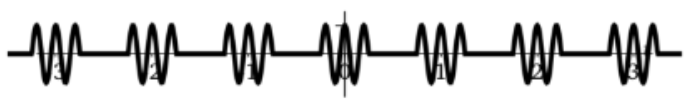
\includegraphics[scale=0.8]{W2_2.png}
\end{center}
How do we write this using the step function as a building block?  Each burst have a form of $A \cos(\omega t)$ and last for a width 0.5 around each integer.\\\\
\textbf{Solution:\\}
The burst around 0 can be written as 
\[rect(2t) \cdot A \cos(\omega t)\]
The burst around 1 can be written as
\[rect(2(t - 1)) \cdot A \cos(\omega t)\]
and et cetera.  As a result, we can write the entire function as:
\[y(t) = \sum_{i = -\infty}^{\infty} rect(2(t - i)) \cdot A\cos(\omega t)\]
\subsection*{Unit Ramp}
The unit ramp is defined as:
\[r(t) = \begin{cases}t & t \geq 0 \\ 0 & t < 0 \end{cases}\]
Note that the unit ramp is the integral of the unit step, i.e.
\[r(t) = \int_{-\infty}^t u(r) \text{d}r\]
The unit ramp is illustrated below:
\begin{center}
    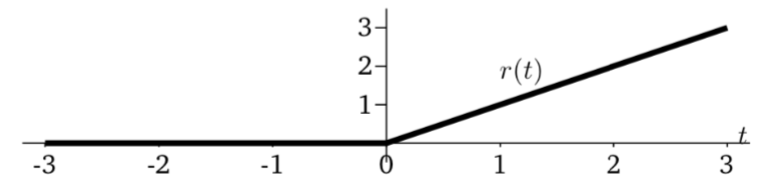
\includegraphics[scale=0.8]{W2_3.png}
\end{center}
This is known in the AI world as ReLU().
\subsubsection*{Unit Triangle}
The unit triangle is defined as:
\[\triangle(t) = \begin{cases}1 - \vert t \vert & \vert t \vert < 1 \\ 0 & \text{else}\end{cases}\]
The unit triangle is illustrated below:
\begin{center}
    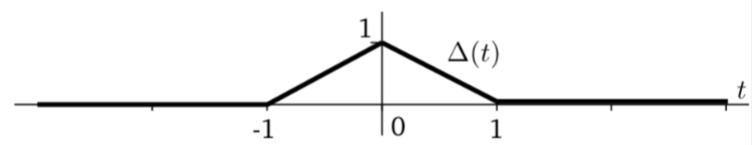
\includegraphics[scale=0.5]{W2_4.png}
\end{center}
\example\\
Lets say we want to make a skewed triangle.  
\begin{center}
    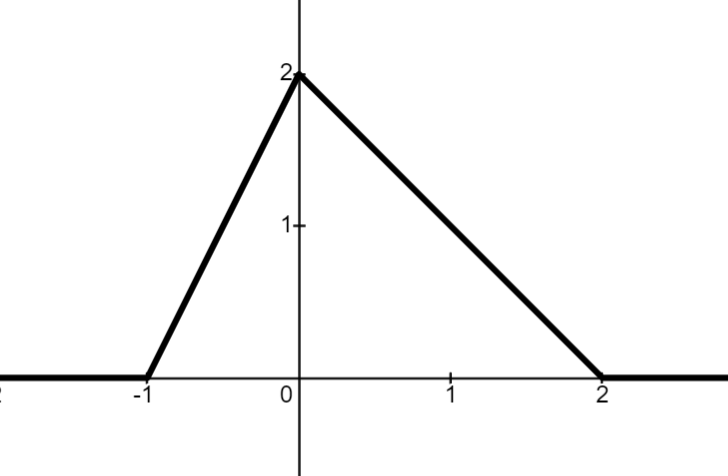
\includegraphics[scale=0.5]{W2_5.png}
\end{center}
\textbf{Solution:\\}
\[x(t) = 2\triangle(t) + \triangle(t - 1)\]
The intuition is the following:
\begin{center}
    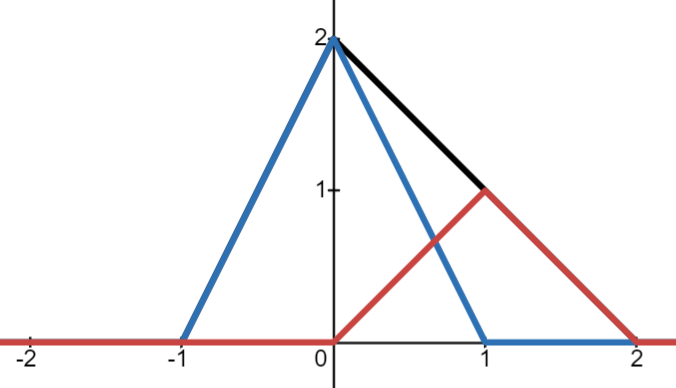
\includegraphics[scale=0.5]{W2_6.png}
\end{center}
The $2\triangle(t)$ term represents the blue line and the $\triangle(t - 1)$ term represents the red line.  We can add the two lines between $0 \geq t \geq 1$ to get the negative 1 slope we need.

\subsection*{Impulse Function}
\textbf{This is an extremely important signal.}
\begin{itemize}
    \item This is defined as $\delta(t)$, or "impulse", "delta", or "Dirac" function.  It is \textbf{not} a rigorous mathematical function.
    \item Features of the impulse function:
    \begin{enumerate} 
        \item It is very large (i.e., approaching infinity), at $t = 0$
        \item It's zero everywhere else, $t \neq 0$.
        \item Area = 1
    \end{enumerate}
    \item Shown on the graph as an arrow pointing up at $t = 0$
\end{itemize}
\begin{center}
    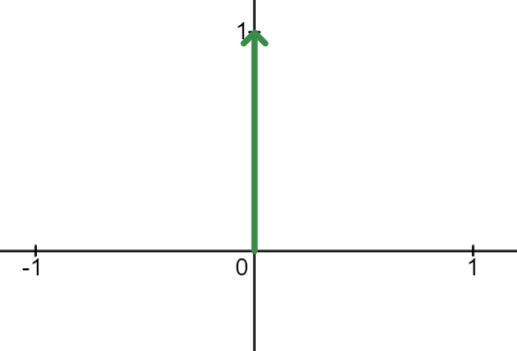
\includegraphics[scale=0.5]{W2_7.png}
\end{center}
\begin{itemize}
    \item The intuition of the impulse function is a $rect_{\Delta}(t)$ where $\Delta$ approaches 0.  (e.g., the width of the rectangle goes to 0 and the height goes to infinity.)
    \item $\delta(t) \cdot x(t) = x(0) \cdot \delta(t)$, where $x(t)$ is any function.
    \begin{itemize}
        \item The impulse is still affected by other functions because by intuition it is a very, very thin rectangle.  The height is an infinitely large number, but not infinity.
        \item The area of the impulse is also scaled by $x(0)$.
        \item The shape of the impulse does not change with scaling, but its area does.
        \item This is called the \textbf{impulse dampening property}.
    \end{itemize}
    \item The impulse can be moved by an amount $T$:
    \[x(t) \cdot \delta(t - T) = x(T) \cdot \delta(t - T)\]
    \begin{itemize}
        \item This is called the \textbf{impulse sampling property}.
    \end{itemize}
    \item What happens when we take the integral?
    \begin{align*}
        &\int_{-\infty}^\infty x(t) \cdot \delta(t) \text{d}t\\
        = &\int_{-\infty}^\infty x(0) \cdot \delta(t) \text{d}t\\
        = &\:x(0) \cdot \int_{-\infty}^\infty \delta(t) \text{d}t\\
        = &\:x(0)
    \end{align*}
    \item What if it is shifted?
    \begin{align*}
        &\int_{-\infty}^\infty x(t) \cdot \delta(t - T) \text{d}t\\
        = &\int_{-\infty}^\infty x(T) \cdot \delta(t - T) \text{d}t\\
        = &\:x(T) \cdot \int_{-\infty}^\infty \delta(t - T) \text{d}t\\
        = &\:x(T)
    \end{align*}
    \[\boxed{\int_{-\infty}^\infty x(t) \delta(t - T) \text{d}t = x(T)}\]
    \begin{itemize}
        \item This is called the \textbf{impulse sifting property}.
    \end{itemize}
\end{itemize}
\subsubsection*{Integral of an impulse}
\begin{align*}
    \int_{\infty}^\infty \delta(t) \text{d}t &= 1\\
    \int_{\infty}^{0+} \delta(t) \text{d}t &= 1\\
    \int_{\infty}^{0-} \delta(t) \text{d}t &= 0
\end{align*}
The $0+$ represents approaching zero from the right (e.g., infinitely close to zero on the positive side), and $0-$ represents approaching zero on the left (e.g., infinitely close to zero on the negative side).

\end{document}
